\documentclass[12pt,a4paper]{article}

% ==== Packages ====
\usepackage{geometry}
\usepackage{graphicx}
\usepackage{setspace}
\usepackage{fancyhdr}
\usepackage{listings}
\usepackage{xcolor}
\usepackage{titlesec}
\usepackage{pgfplots}
\usepackage{pgf-pie}
\usepackage{caption}

% ==== Page Setup ====
\geometry{margin=1in}
\setstretch{1.5}
\pagestyle{fancy}
\fancyhead[L]{Library Management System}
\fancyhead[R]{Page \thepage}
\fancyfoot{}

% ==== Code Styling ====
\definecolor{codegray}{rgb}{0.5,0.5,0.5}
\definecolor{backcolour}{rgb}{0.95,0.95,0.92}

\lstdefinestyle{mystyle}{
    backgroundcolor=\color{backcolour},   
    commentstyle=\color{gray},
    keywordstyle=\color{blue},
    numberstyle=\tiny\color{codegray},
    stringstyle=\color{purple},
    basicstyle=\ttfamily\footnotesize,
    breaklines=true,
    captionpos=b,
    numbers=left,
    numbersep=5pt,
    showspaces=false,
    showstringspaces=false,
    tabsize=2
}
\lstset{style=mystyle}

% ==== Title Section ====
\title{\textbf{Library Management System}\\[5pt]\large A Python Console Project}
\author{}
\date{}

\begin{document}

\maketitle
\thispagestyle{empty}

\vspace{1cm}
\begin{center}
\textbf{Submitted by:}\\[4pt]
Team of Three Members\\
Under Toolkit for Research Project
\end{center}

\newpage

% ==== Table of Contents ====
\tableofcontents
\newpage

% ==== Sections ====
\section{Introduction}
The Library Management System is a simple Python-based console application designed to manage a collection of books. It allows users to add, view, search, and delete book records, ensuring that data is stored persistently using a JSON file. 

This project demonstrates the use of Python’s core concepts like functions, file handling, and modular programming.

\section{Objective}
\begin{itemize}
    \item To provide a basic and easy-to-use system for library data management.
    \item To apply Python programming concepts such as file handling, data structures, and modular coding.
    \item To help students understand how to split a project among multiple team members using GitHub.
\end{itemize}

\section{Team Division}
\begin{center}
\begin{tabular}{|l|l|}
\hline
\textbf{Member} & \textbf{Files Assigned} \\ \hline
Member 1 & main.py, book\_operations.py \\ \hline
Member 2 & manage\_books.py, helpers.py \\ \hline
Member 3 & storage.py, utils.py \\ \hline
\end{tabular}
\end{center}

\section{System Design}
The system is menu-driven and allows users to:
\begin{enumerate}
    \item Add a new book with title, author, and year.
    \item View all existing books.
    \item Search for a book by title or author.
    \item Delete a book using its unique ID.
    \item Save all records into a JSON file.
\end{enumerate}

\section{Code Implementation}
Below are key code snippets from the project.

\subsection{Main Menu (main.py)}
\begin{lstlisting}[language=Python, caption=main.py]
from book_operations import add_book, view_books
from manage_books import search_book, delete_book
from storage import save_data, load_data

def main():
    books = load_data()

    while True:
        print("\n=== Library Management System ===")
        print("1. Add Book")
        print("2. View Books")
        print("3. Search Book")
        print("4. Delete Book")
        print("5. Save & Exit")

        choice = input("Enter your choice: ")

        if choice == '1':
            add_book(books)
        elif choice == '2':
            view_books(books)
        elif choice == '3':
            search_book(books)
        elif choice == '4':
            delete_book(books)
        elif choice == '5':
            save_data(books)
            print("Data saved! Exiting...")
            break
        else:
            print("Invalid choice, try again!")
\end{lstlisting}

\subsection{Book Operations (book\_operations.py)}
\begin{lstlisting}[language=Python, caption=book_operations.py]
from utils import generate_id

def add_book(books):
    title = input("Enter book title: ")
    author = input("Enter author name: ")
    year = input("Enter publication year: ")
    book_id = generate_id()

    book = {"id": book_id, "title": title, "author": author, "year": year}
    books.append(book)
    print("Book added successfully!")

def view_books(books):
    if not books:
        print("No books found in the library.")
        return
    for b in books:
        print(f"ID: {b['id']} | {b['title']} by {b['author']} ({b['year']})")
\end{lstlisting}

\section{Data Visualization}
The following charts show example data analysis from the library system.

\subsection{Bar Graph — Number of Books by Year}
\begin{center}
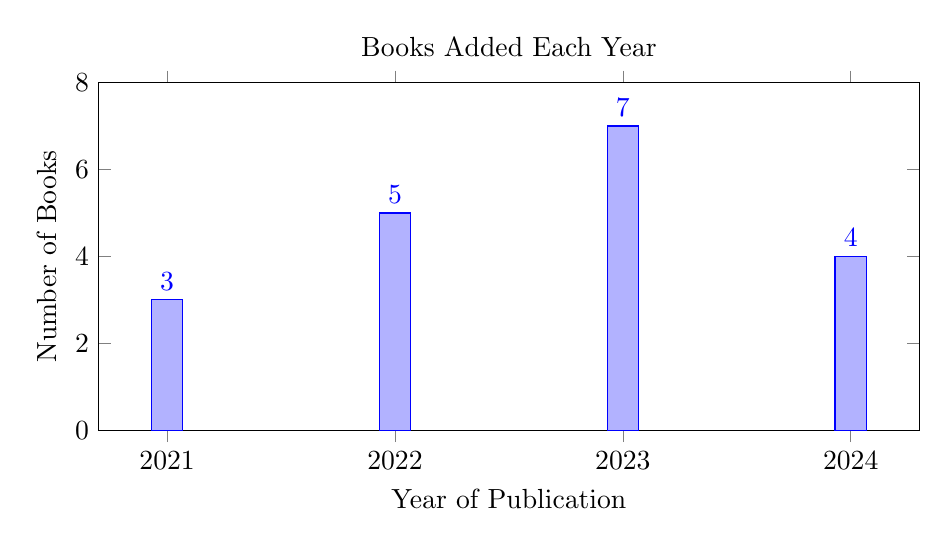
\begin{tikzpicture}
\begin{axis}[
    ybar,
    xlabel={Year of Publication},
    ylabel={Number of Books},
    ymin=0, ymax=8,
    bar width=0.4cm,
    width=12cm,
    height=6cm,
    symbolic x coords={2021,2022,2023,2024},
    xtick=data,
    nodes near coords,
    title={Books Added Each Year}
]
\addplot coordinates {(2021,3) (2022,5) (2023,7) (2024,4)};
\end{axis}
\end{tikzpicture}
\captionof{figure}{Bar graph showing number of books added per year.}
\end{center}

\subsection{Pie Chart — Distribution of Books by Author}
\begin{center}
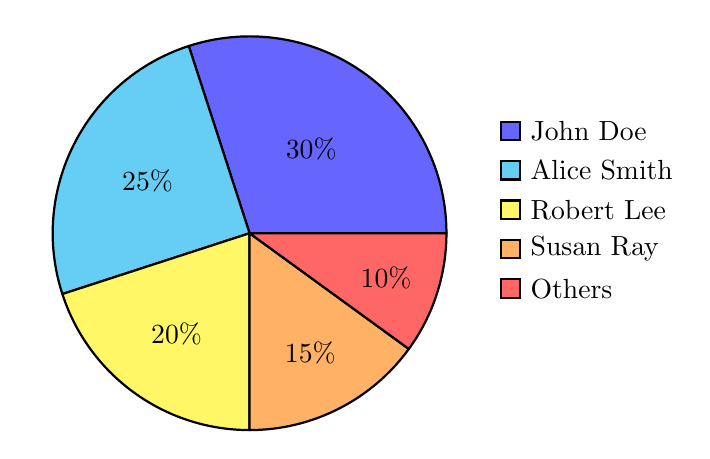
\begin{tikzpicture}
\pie[text=legend, radius=2.5]{
30/John Doe,
25/Alice Smith,
20/Robert Lee,
15/Susan Ray,
10/Others
}
\end{tikzpicture}
\captionof{figure}{Pie chart showing distribution of books by author.}
\end{center}

\section{Results}
The program successfully performs:
\begin{itemize}
    \item Adding and viewing books.
    \item Searching and deleting by ID.
    \item Storing data persistently using JSON.
\end{itemize}

\section{Conclusion}
This project demonstrates modular Python programming and team collaboration using Git and GitHub.  
It provided practical experience in handling data, implementing file storage, and presenting visual results.

\section{Future Enhancements}
\begin{itemize}
    \item Add GUI using Tkinter.
    \item Include admin and user login system.
    \item Add book borrowing and return feature.
\end{itemize}

\end{document}
